\section{Beschreibung des Gesamtsystems}
%In diesem Kapitel wird das Gesamtsystem beispielhaft an einem Wagen erläutert. \par
Der neue intelligente \gls{Gueterwagen} soll in Zukunft selbst wissen, was wann mit ihm gemacht wurde, wo er war und welche Wartungszyklen wie eingehalten wurden. Ebenso soll auch eine Überwachung des aktuellen Zustandes und Rückschlüsse auf die Zukunft mittels Sensoren zur vorausschauenden Instandhaltung möglich sein.\par
Des Weiteren  soll er physisch bei der Zugvorbereitung helfen. Erst nur durch aktive Unterstützung bei der Feststellbremse, sodass keine \gls{Hemmschuh}e benötigt werden, Verstellen der \gls{Bremsart}, automatisches Durchführen einer \gls{Bremsprobe} oder Hilfe bei Zugtrennungen. Später aber auch durch ein gewisses Maß an selbstständigem Rangiervermögen.\par
Ebenfalls geplant ist eine digitale Unterstützung bei der Zugvorbereitung. Hier sind vor allem Unterstützungen im Bereich automatische Bremsberechung und \gls{Bremsprobe}, aber auch bei der Zugzusammenstellung geplant.\par
Dafür werden einerseits Sensoren und Aktoren am Wagen angebracht, andererseits auch eine Stromversorgung und ein Bordrechner mit Betriebssystem.\par
Diese Punkte sorgen ebenso für mehr Effizienz in der Zugvorbereitung, nicht nur im Einzelwagenverkehr, auch im Bereich der Ganzzüge und dem Kombinierten Verkehr, die in den Betriebsstätten ebenfalls alleine oder in kleinen Wagengruppen vorbereitet werden, als auch bieten sie angenehmere Arbeitsplätze, bessere Überwachung der Wagen und kosteneffizientere Instandhaltung durch genauere Wartungsintervalle.\par
%Begonnen wird mit der physischen Beschreibung des Güterwagens 4.0. Danach folgt eine Beschreibung des virtuellen Güterwagens im Betriebssystem und der Cloud.\par

\subsection{Der Güterwagen 4.0}
Die einzelnen Komponenten bestehen aus Kombinationen der hier vorgestellten Subsysteme. Darum sollen diese auch hier noch einmal kurz behandelt werden.

\subsubsection{Energieversorgung}
Die dauerhafte Versorgung des \gls{Gueterwagen}s mit Energie stellt ein Novum im Güterver- kehr dar. Vor allem die Nachspeisung der Pufferbatterie durch verschiedene Quellen soll die Akzeptanz erhöhen. In Abbildung \ref{fig:GesSys} ist der \gls{Gueterwagen 40} mit Radsatzgenerator und externer Ladeschnittstelle gezeigt (Kapitel \ref{sec:RSG}). Zusätzlich denkbar sind auch eine Aufladung über die Automatische Kupplung, handgekuppelte Kabelstränge von einem Wagen zum nächsten bei fest verbundenen Wagengruppen, Solarpanels oder sogar Brennstoffzellen. %Diese haben je nach Anwendungsfall alle ihre Zielgruppe.
\par
Die Batterie (Kapitel \ref{sec:Batterie}) speist wiederum sämtliche Aktoren, Sensoren und die Bord- elektronik. Diese Speisung erfolgt sowohl bei der Fahrt zur Aufnahme von Daten der Sensoren sowie der Aktorik der \gls{ep-Bremsen}, als auch bei Stillstand. Hier müssen Lademanagement und Betriebssystem %(Kapitel \ref{sec:Lademanagment}) 
dafür sorgen, dass alle notwendigen Prozesse weiterlaufen, alle Anderen aber heruntergefahren werden, oder die Aktualisierung von Daten seltener erfolgt.


\subsubsection{Bremse 4.0}
Die Bremse des \gls{Gueterwagen 40} bietet folgende Funktionen:
\begin{itemize}
    \item \acrshort{TSI}-konformes Steuerventil mit den \gls{Bremsart}en G und P (Kapitel \ref{sec:Bremsart})
    \item Fernbetätigte Endabsperrhähne (Kapitel \ref{sec:Endabsperrhahn})
    \item Fernbetätigung verschiedener Bremsfunktionen  (Kapitel \ref{sec:Bremsart})
    \begin{itemize}
        \item Schnelllösen
        \item Bremse aus
        \item Bremsstellung
        \item Feststellbremse
        \item \gls{ep-Bremsen}n
        \item Lastabbremsung
    \end{itemize}
    \item Anzeige des Zustands (drucklos, druckbeaufschlagt) der pneumatischen Kupplung (Kapitel \ref{sec:ZustandKupplung})
    \item Messung des C-Drucks (Kapitel \ref{sec:C-Druck})
\end{itemize}


\subsubsection{Bedienen und Beobachten}
Wird von Manfred geschrieben

\subsubsection{Intelligente Vernetzung}
Der \gls{Gueterwagen 40} ist als 'intelligenter' Wagen im Sinne der Industrie 4.0 im Schienenverkehr geplant. Dafür benötigt er, neben der Energieversorgung und der teilautomatisierten Bremse, auch einen Bordrechner, der diese 'Intelligenz' liefert.\par
Auf diesem Rechner soll als Betriebssystem das sogenannte '\gls{WagonOS}' installiert sein. Dieses bietet als Open Source-System ein offenes Betriebssystem mit vielen Ausbaumög- lichkeiten. Das \gls{WagonOS} bietet den Nutzern des \gls{Gueterwagen 40} diesen auf genau die benötigten Anwendungsfälle zu Optimieren und sogar die Möglichkeit eigene Applikationen zu erstellen.\par
Des Weiteren liegen auf dieser Speichereinheit dezentral alle für die Zugbildung und Instandhaltung wichtigen Informationen über den Wagen. Dazu gehören bauartspezifische Parameter wie Gewicht, Länge, Achszahl, maximal Zuladung und Höchstgeschwindigkeit genauso wie wagenspezifische Informationen wie Besitzer, Laufleistung, Informationen aus den Sensoren, letzte Wartungen und nächste Instandhaltungszyklen.\par
Diese Informationen liegen ebenso als 'Digitaler Zwilling' in einer Cloud. Bei Verbindung des Wagens zum Internet und Änderung der Informationen auf dem Wagen wird dieser Zwilling regelmäßig aktualisiert.\par
Im Verband mit anderen Wagen verhält sich der \gls{Gueterwagen 40} 'sozial' und teilt alle notwendigen Informationen über sich mit den anderen Wagen und der Lok als gleichberechtigte Partner. Durch die Verbindung von Wagen zu Wagen ist keine durchgehende Internetverbindung notwendig. Die Informationen können lokal ausgetauscht und später synchronisiert werden.\par
Im Projekt umgesetzt werden soll davon eine reduzierte Form des \gls{WagonOS}. Eine Entwicklung des vollständigen Betriebssystems findet nicht im Rahmen dieses Projektes statt.\par
Diese reduzierte Form des Betriebssystems soll eine Speicherung und Auswertung aller relevanter Daten auf dem Bordrechner ermöglichen. Eine weitere Datenspeicherung als 'Digitaler Zwilling' findet in der Cloud statt.



\subsection{Physischer Güterwagen 4.0}
Das Gesamtsystem, bestehend aus elektrischer, pneumatischer, sensorischer und Datenkomponenten ist in der Abbildung \ref{fig:GesSys} zu sehen.\par
    \begin{figure}[hbt]
        \centering
    \pgfdeclarelayer{background}
\pgfdeclarelayer{foreground}
\pgfdeclarelayer{Beschriftung}
%Farbendefinition
\definecolor{elek}{RGB}{55,126,184}%blau
\definecolor{pneu}{RGB}{77,175,74}%grün
\definecolor{sens}{RGB}{228,26,28}%rot
\definecolor{dat}{RGB}{152,78,163}%violet
\definecolor{strom}{RGB}{0,0,0}%schwarz

\tikzset{wagon/.style={draw = gray, ultra thick, opacity = 0.7}}
\tikzset{seite/.style={opacity = 1}}
\tikzset{elek/.style= {draw = elek, ultra thick, opacity = 1}} %elektrische Komponenten
\tikzset{sens/.style={draw = sens, ultra thick, opacity = 1}} %sensorische Komponenten
\tikzset{pneu/.style={draw = pneu, ultra thick, opacity = 1}} %pneumatische Komponenten
\tikzset{dat/.style={draw = dat, ultra thick, opacity = 1}} %Datenkomponenten
\tikzset{strom/.style={draw = strom, ultra thick, opacity = 1}} %Strom- und Datenleitungen
\tikzset{annotation/.style={draw = black, thick, opacity = 0.7, font=\scriptsize}}

\pgfsetlayers{background,main,Beschriftung,foreground}
\begin{tikzpicture}[scale=0.6]
%%%%%%%%%%%%%%%%%%%%%%%%%%%%%%%%%%%%%%%%%%%%%%%% Hintergrund %%%%%%%%%%%%%%%%%%%%%%%%%%%%%%%%%%%%%%%%%%%%%
    \begin{pgfonlayer}{background}
    %Seiten
        %Seite A
        \path[seite] (0, 3) rectangle +(.6,.2) node[pos = 0.5] (seiteA) {Seite A};
        %Seite B
        \path[seite] (0, -3.2) rectangle +(.6,.2) node[pos = 0.5] (seiteB) {Seite B};
        %Seite 1
        \path[seite] (-12.3, 0) rectangle +(.6,.2) node[pos = 0.5] (seiteB) {Seite 1};
        %Seite 2
        \path[seite] (10.3, 0) rectangle +(.6,.2) node[pos = 0.5] (seiteB) {Seite 2};      
    %wagon als Basis
    \path[wagon] (-5,-2) -- (-5,2) -- (5,2) -- (5,-2) -- cycle;
    % HL
    \path[wagon, color=pneu] (-5,-.5) -- (5,-.5) node[pos = 0.6, above] {\color=\gray \tiny{HL}};
    % Buffer
    \begin{scope}[shift = {(-5,1.5)}]
    	\path[wagon] (-.8,.3) -- (0,.3) -- (0,-.3) -- (-.8,-.3);
    	\path[wagon] (-1,.25) -- (-.8,.25) -- (-.8,-.25) -- (-1,-.25);
    	\path[wagon] (-1,-.5) .. controls (-1.05,0) and (-1.05,0) .. (-1,.5);
    \end{scope}
    \begin{scope}[shift = {(-5,-1.5)}]
    	\path[wagon] (-.8,.3) -- (0,.3) -- (0,-.3) -- (-.8,-.3);
    	\path[wagon] (-1,.25) -- (-.8,.25) -- (-.8,-.25) -- (-1,-.25);
    	\path[wagon] (-1,-.5) .. controls (-1.05,0) and (-1.05,0) .. (-1,.5);
    \end{scope}
    \begin{scope}[shift = {(5,-1.5)}, rotate = 180]
    	\path[wagon] (-.8,.3) -- (0,.3) -- (0,-.3) -- (-.8,-.3);
    	\path[wagon] (-1,.25) -- (-.8,.25) -- (-.8,-.25) -- (-1,-.25);
    	\path[wagon] (-1,-.5) .. controls (-1.05,0) and (-1.05,0) .. (-1,.5);
    \end{scope}
    \begin{scope}[shift = {(5,1.5)}, rotate = 180]
    	\path[wagon] (-.8,.3) -- (0,.3) -- (0,-.3) -- (-.8,-.3);
    	\path[wagon] (-1,.25) -- (-.8,.25) -- (-.8,-.25) -- (-1,-.25);
    	\path[wagon] (-1,-.5) .. controls (-1.05,0) and (-1.05,0) .. (-1,.5);
    \end{scope}
    %Wheelset
    \begin{scope}[shift = {(-4,0)}]
    	\path[wagon] (-.1,1.7) -- (.1,1.7) -- (.1,-1.7) -- (-.1, -1.7) -- cycle; 
    	\path[wagon] (-.6,1.4) -- (.6,1.4) -- (.55,1.5) -- (-.55, 1.5) -- cycle; 
    	\path[wagon] (-.6,-1.4) -- (.6,-1.4) -- (.55,-1.5) -- (-.55, -1.5) -- cycle; 
    \end{scope}
        \begin{scope}[shift = {(-2.5,0)}]
    	\path[wagon] (-.1,1.7) -- (.1,1.7) -- (.1,-1.7) -- (-.1, -1.7) -- cycle; 
    	\path[wagon] (-.6,1.4) -- (.6,1.4) -- (.55,1.5) -- (-.55, 1.5) -- cycle; 
    	\path[wagon] (-.6,-1.4) -- (.6,-1.4) -- (.55,-1.5) -- (-.55, -1.5) -- cycle; 
    \end{scope}
    \begin{scope}[shift = {(4,0)}]
    	\path[wagon] (-.1,1.7) -- (.1,1.7) -- (.1,-1.7) -- (-.1, -1.7) -- cycle; 
    	\path[wagon] (-.6,1.4) -- (.6,1.4) -- (.55,1.5) -- (-.55, 1.5) -- cycle; 
    	\path[wagon] (-.6,-1.4) -- (.6,-1.4) -- (.55,-1.5) -- (-.55, -1.5) -- cycle; 
    \end{scope}
    \begin{scope}[shift = {(2.5,0)}]
    	\path[wagon] (-.1,1.7) -- (.1,1.7) -- (.1,-1.7) -- (-.1, -1.7) -- cycle; 
    	\path[wagon] (-.6,1.4) -- (.6,1.4) -- (.55,1.5) -- (-.55, 1.5) -- cycle; 
    	\path[wagon] (-.6,-1.4) -- (.6,-1.4) -- (.55,-1.5) -- (-.55, -1.5) -- cycle; 
    \end{scope}
    \end{pgfonlayer}
%%%%%%%%%%%%%%%%%%%%%%%%%%%%%%%%%%%%%%%%%%%%%%% Vordergrung %%%%%%%%%%%%%%%%%%%%%%%%%%%%%%%%%%%%%%%%%%%%%%%%%
    \begin{pgfonlayer}{foreground} %Komponete
    %elektronische Komponenten
        %Radsatzgenerator
        \path[elek, fill = elek, thin] (-4.3, -1.9) rectangle +(.6,.2) node[pos = 0.5] (wsg) {};
        %Rechner
        \path[elek, fill = elek, thin] (-.5, -1.6) rectangle +(1,.3) node[pos = 0.5] (bcu) {};
        %Batterie
        \path[elek, fill = elek, thin] (-1.8, -1.8) rectangle +(1,.5) node[pos = 0.5] (bat) {};
        %optionale Ladeelektronik
        \path[elek, fill = elek, thin] (-1.8, 1.2) rectangle +(0.8,.4) node[pos = 0.5] (ole) {};
    % pneumatische Komponenten
        %epBremse
        \path[pneu, fill = pneu] (.9,-1.3) rectangle (1.1,-1.5) node[pos = 0.5] (epb) {};
        %Endabsperrhähne
        \path[pneu, fill = pneu] (-5.2, -.4) rectangle (-5,-.6) node[pos = 0.5] (eca) {};
        \path[pneu, fill = pneu] (5.2, -.4) rectangle (5,-.6) node[pos = 0.5] (ecb) {};
        %Aktorik Bremse
        \path[pneu, fill = pneu, thin] (-.5, 0) rectangle +(1,.5) node[pos = 0.5] (bcu2) {};
    %sensorische Komponenten
        %drahtloserSensor
        \path[sens, fill = sens, thin] (3.9, -1.7) rectangle +(.2,-.2) node[pos = 0.5] (wss) {};
        %Flachstellendektektor
        \path[sens, fill=sens, thin] (3.15, 1.8) rectangle +(.2,-.2) node[pos = 0.5] (flachstelle) {};
        \path[sens, fill=sens, thin] (-3.35, 1.8) rectangle +(.2,-.2) node[pos = 0.5] (flachstelle2) {};
        %Laufleistung
        \path[sens, fill = sens, thin] (3.9, 0) rectangle +(.2,-.2) node[pos = 0.5] (ll) {};
    %Datenkomponeten
        %Kurzstreckenfunk
        \path[dat, fill = dat] (-5.2, -.9) rectangle (-5,-1.05)node[pos = 0.5] (sra) {};
        \path[dat, fill = dat] (5.2, -.9) rectangle (5,-1.05)node[pos = 0.5] (srb) {};
        \path[dat, fill = dat] (5.2, .9) rectangle (5,1.05)node[pos = 0.5] (src) {};
        \path[dat, fill = dat] (-5.2, .9) rectangle (-5,1.05) node[pos = 0.5] (srd) {};
    \end{pgfonlayer}
%%%%%%%%%%%%%%%%%%%%%%%%%%%%%%%%%%%%%%%%%%%%%%% Beschriftung %%%%%%%%%%%%%%%%%%%%%%%%%%%%%%%%%%%%%%%%%%%%%%%%%
    \begin{pgfonlayer}{Beschriftung}
    %elektronische Komponenten
        %Radsatzgenerator
        \path[annotation, thin] (wsg) -- +(-.5,-.5) node[left] {Radsatzgenerator};
        %Rechner
        \path[annotation, thin] (bcu) -- +(1,-1) node[right] {Bordelektronik};
        %Batterie
        \path[annotation, thin] (bat) -- +(-1,-1) node[left] {Batterie};
        %optionale Ladeelektronik
        \path[annotation, thin] (ole) -- +(-.9,.9) node[left] {externe Ladeschnittstelle};
    %pneumatische Komponenten
        %epBremse
        \path[annotation, thin] (epb) -- +(.4,-.4) node[right] {ep-Bremse};
        %Endabsperrhähne
        \path[annotation, thin] (eca) -- +(-.5,.5) node[left] {Aktor Endabsperrhahn};
        %Aktorik Bremse
        \path[annotation, thin] (bcu2) -- +(.5,.5) node[right] {Aktorik Bremse};
    %sensorische Komponenten
        %drahtloserSensor
        \path[annotation, thin] (wss) -- +(.5,-.5) node[right] {Laufleistung}; 
        %Flachstellen
        \path[annotation, thin] (flachstelle) -- +(.7,.7) node[right] {Lagertemperatur};
        \path[annotation, thin] (flachstelle2) -- +(7.2,.7) node[right] {};
        %Laufleistung
        \path[annotation, thin] (ll) -- +(1.2,.5) node[right] {Beschleunigungen};
    %Datenkomponeten
        %Kurzstreckenfunk
        \path[annotation, thin] (srd) -- +(-.5,-.5) node[left] {Kurzstreckenfunk};    
    \end{pgfonlayer}
%%%%%%%%%%%%%%%%%%%%%%%%%%%%%%%%%%%%%%%%%%%%%% Main %%%%%%%%%%%%%%%%%%%%%%%%%%%%%%%%%%%%%%%%%%%%%%%%%%%%
    \begin{pgfonlayer}{main} %Leitungen
    %elek
        %Radsatzgenerator
        \path[elek] (wsg) +(-.1,0) -| (-3.3, -1);%-- +(1,0) -- (-3.2,-1);
        \path[strom, dashed] (wsg) +(-.1,0) -| (-3.3, -1);%-- +(1,0) -- (-3.2,-1);
        %Rechner
        \path[elek] (bcu) +(0,0)  -- (0,-1);
        \path[strom, dashed] (bcu) +(0,0)  -- (0,-1);
        %Batterie
        \path[elek] (bat) +(0,0)  -- (-1.3,-1);
        \path[strom, dashed] (bat) +(0,0)  -- (-1.3,-1);
        %optionale Ladeelektronik
        \path[elek] (ole) +(0,0)  -- (-1.35,-1);
        \path[strom, dashed] (ole) +(0,0)  -- (-1.35,-1);
    %pneu
        %ep-Bremse
        \path[pneu] (1,-.5) -- (1,-1.3);
        %\path[strom, dashed] (1,-.5) -- (1,-1.3);
        \path[pneu] (epb) +(.1,0) -- +(-.5,0);
        \path[strom, dashed] (epb) +(.1,0) -- +(-.5,0);
        %Endabsperrhähne
        \path[pneu] (eca) +(-.1,0) -- +(.2,0) -- (-4.9,-1);
        \path[strom, dashed] (eca) +(-.1,0) -- +(.2,0) -- (-4.9,-1);
        \path[pneu] (ecb) +(.1,0) -- +(-.2,0) -- (4.9,-1);
        \path[strom, dashed] (ecb) +(.1,0) -- +(-.2,0) -- (4.9,-1);
        %Aktorik Bremse
        \path[pneu] (bcu2) +(0,0)  -- (0,-1);
        \path[strom, dashed] (bcu2) +(0,0)  -- (0,-1);
    %Sensorische Kompoenten
        %Flachstellen
        \path[sens] (flachstelle)+(0,0) -- (3.2, -1);
        \path[strom, dashed] (flachstelle)+(0,0) -- (3.2, -1);
        \path[sens] (flachstelle2) +(0,0)-- (-3.3, -1);
        \path[strom, dashed] (flachstelle2) +(0,0)-- (-3.3, -1);
        %Laufleistung
        \path[sens] (ll)+(0,0) -- (4, -1);
        \path[strom, dashed] (ll)+(0,0) -- (4, -1);
        %drahloser Sensor
        \path[strom, dotted] (wss)+(0,0) -- (4, -1);
    %Strom- und Datenleitung
        \path[dat] (-5,-1) -- (5,-1);
        \path[strom, dashed] (-5,-1) -- (5,-1);
        %Kurzstreckenfunk
        \path[dat] (srd) +(-.1,0) -- +(.3,0) -- (-4.8,-1);
        \path[strom, dashed] (srd) +(-.1,0) -- +(.3,0) -- (-4.8,-1);
        \path[dat] (src) +(.1,0) -- +(-.3,0) -- (4.8,-1);
        \path[strom, dashed] (src) +(.1,0) -- +(-.3,0) -- (4.8,-1);
    \end{pgfonlayer}

\end{tikzpicture}

        \caption{Zusätzliche Komponenten des Gesamtsystems}
        \label{fig:GesSys}
    \end{figure}
Abgebildet ist im Hintergrund in grau ein gebremster, vier-achsiger (in zwei Drehgestellen) \gls{Gueterwagen}, mit Puffern und Schraubenkupplung. Eine genaue Bauart ist und soll nicht erkennbar sein. Die elektrischen Komponenten sind in blau, die pneumatischen Komponenten in grün, die sensorischen Komponenten in rot und die Datenkomponenten in violett eingefärbt. Zusätzlich sind die Elemente, die mit Strom versorgt werden auch mit einer schwarzen, gestrichelten Linie verbunden.\par
Das Konzept des \gls{Gueterwagen}s besteht aus vier großen Unterpunkten, die hier beschrieben werden.
\begin{itemize}
    \item Stromversorgung des \gls{Gueterwagen}s,
    \item Teilautomatisierung des \gls{Gueterwagen}s durch Aktoren,
    \item Zustandsüberwachung des \gls{Gueterwagen}s durch Sensoren und
    \item Intelligenter Vernetzung zwischen \gls{Gueterwagen} und weiteren Bahnanlagen.
\end{itemize}
Diese Punkte werden in folgenden Unterkapiteln einzeln beleuchtet. Nach einer Beschreibung des virtuellen \gls{Gueterwagen}s folgt die Stromversorgung mit ihren Komponenten, anschließend erfolgt eine Ausführung über pneumatische Komponenten, die der Teilautomatisierung durch Aktoren entspricht. Im Anschluss folgt ein Kapitel über die Zustandsüberwachung mittels Sensorik und später eine Ausführung über die Systeme, die dem Wagen 'Intelligenz' bieten sollen.

\subsection{Virtueller Güterwagen 4.0}
Für eine, wie die bereits beschriebene, intelligente Vernetzung der \gls{Gueterwagen} wird nicht nur ein physischer \gls{Gueterwagen} mit Sensoren und Aktoren sowie deren Auswertung benötigt, sondern auch eine Kommunikationsmöglichkeit. Für diese wird eine virtuelle Entsprechung des \gls{Gueterwagen}s benötigt: der virtuelle \gls{Gueterwagen 40}.\par
Jeder \gls{Gueterwagen 40} besitzt einen 'Digitalen Zwilling'. In ihm werden alle Zustände und Aktorstellungen gespeichert. Siehe dazu auch \ref{sec:dKomp}. Für die Speicherung der Daten und Kommunikation mit anderen Wagen wird das bereits angesprochene Betriebssystem '\gls{WagonOS}' benötigt.\par
Die Architektur dieser offenen \gls{Gueterwagen}-Software stützt sich auf folgende Punkte:
\begin{itemize}
    \item Internettechnologien
    \item IPv6-basiert
    \item Dezentral
    \item Zukunftssicher
\end{itemize}
Durch die Wahl von Internettechnologien sind beliebige Übertragungsmöglichkeiten wähl- bar und kombinierbar.\par
Durch eine Basierung auf IPv6 ist eine eindeutige Identifizierung jedes Wagens möglich. Zur eindeutigen Zuordnung soll die UIC-Wagennummer auch der Netzwerkadresse entsprechen. Siehe dazu auch Abbildung \ref{fig:IPv6}.\par
\begin{figure}
    \centering
    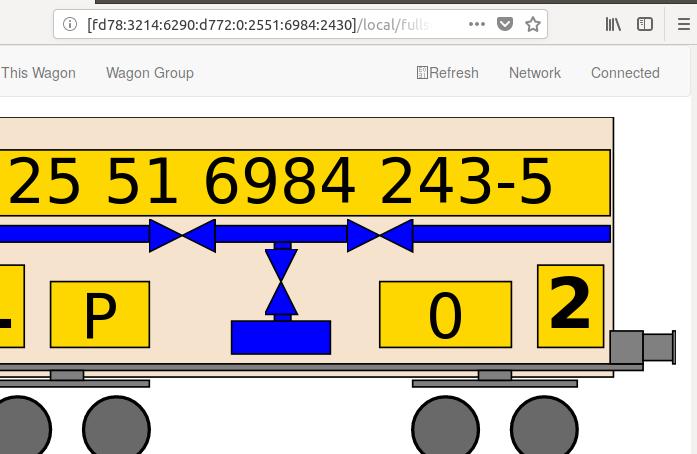
\includegraphics[width=\textwidth]{Bilder/ipv6_concept.png}
    \caption{Mögliche Darstellung des virtuellen \gls{Gueterwagen}s mit IPv6-Netzwerkadresse\cite{GAK}}
    \label{fig:IPv6}
\end{figure}
Alle Wagen sollen hierarchisch gleich gestellt sein. außerdem darf keine Abhängigkeit zu Netzwerkverbindungen oder Servern bestehen. Darum soll durch Dezentralität und lokalen Netzwerken immer eine lokale Verbindung bestehen. In dieser wird eine lokale Hierarchie gebildet.\par
Im Verband mit anderen Wagen verhält sich der \gls{Gueterwagen 40} sozial und teilt alle notwendigen Informationen über sich mit den anderen Wagen und der Lok als gleichberechtigte Partner. Dazu gehören bauartspezifische Parameter wie Gewicht, Länge, Achszahl, maximal Zuladung und Höchstgeschwindigkeit genauso wie wagenspezifische Informationen wie Besitzer, Laufleistung, Informationen aus den Sensoren, letzte Wartungen und nächste Instandhaltungszyklen.\par
Aufgrund der vielen unterschiedlich konfigurierten \gls{Gueterwagen} und Zugängen zu Daten und Akten wird eine NoSQL-Technologie als Datenbankformat gewählt. Diese sorgt auch bei unterschiedlichen Versionen und Daten für eine zukunftssichere Datenbank.\par
Eine weitere Beschreibung des Bordrechners ist in Kapitel \ref{sec:eKomp} zu finden, die Beschreibung der Kommunikation in Kapitel \ref{sec:dKomp} zu finden.
